\documentclass[tikz,border=8pt]{standalone}
\usepackage{amsmath}
\usepackage{amssymb}
\usetikzlibrary{arrows.meta,calc,decorations.pathreplacing,patterns,shapes.geometric,positioning,shadings,plotmarks}

\begin{document}
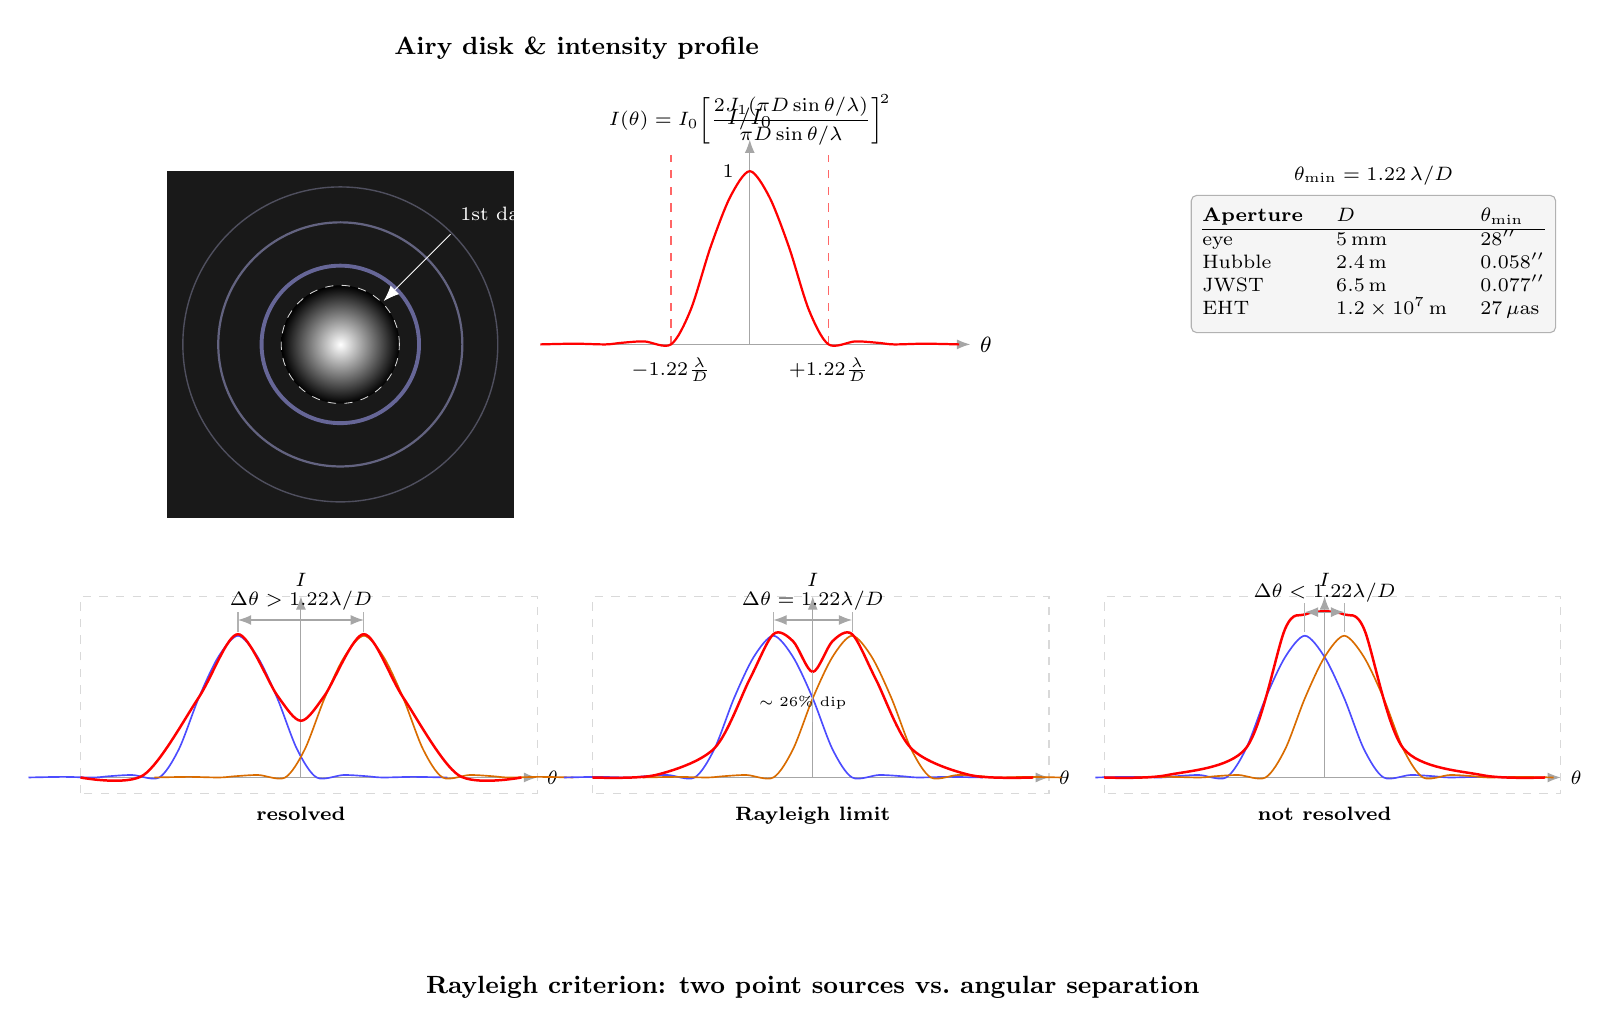
\begin{tikzpicture}[>=Latex]

% ============================================================
%  TOP SECTION: Airy disk image + horizontal intensity profile
% ============================================================

% ---- Airy disk image (circular shaded + faint rings) ----
% Center of Airy disk
\coordinate (A) at (0,0);

% Outer faint box background (subtle)
% First draw a dark background square to represent focal plane
\fill[black!90] (-2.2,-2.2) rectangle (2.2,2.2);

% Central bright disk (radius 0.7 represents theta = 1.22 lambda/D)
% Use radial shading from white/cyan to black
\shade[inner color=white, outer color=black] (A) circle (0.75);

% First bright ring (small annulus) around disk: peak ~1.63 lambda/D
\draw[blue!35, line width=1.4pt, opacity=0.55] (A) circle (1.0);
% Second bright ring: peak ~2.68 lambda/D  -> radius ratio 2.68/1.22 = 2.2
\draw[blue!25, line width=0.8pt, opacity=0.45] (A) circle (1.55);
% Third ring (very faint)
\draw[blue!20, line width=0.5pt, opacity=0.30] (A) circle (2.0);

% First dark ring marker (dashed white circle) at radius 0.75 (== 1.22 l/D scale)
\draw[white, dashed, line width=0.3pt, opacity=0.85] (A) circle (0.75);

% Label for Airy disk image
\node[white, font=\footnotesize] at (0,-2.5) {Airy disk};
\node[white, font=\scriptsize] at (0,2.5) {$\theta = 1.22\,\lambda/D$};

% Arrow pointing to first dark ring
\draw[-{Latex[length=2mm]}, white, line width=0.3pt]
    (1.4,1.4) -- (0.55,0.55);
\node[white, font=\scriptsize, anchor=south west] at (1.4,1.4) {1st dark ring};

% ---- Intensity profile I(theta) on the right ----
% Place origin of plot
\begin{scope}[xshift=5.2cm, yshift=0cm]
% Axes
\draw[->, gray!70] (-2.6,0) -- (2.8,0) node[right, black, font=\footnotesize] {$\theta$};
\draw[->, gray!70] (0,0) -- (0,2.6) node[above, black, font=\footnotesize] {$I/I_0$};

% Tick for peak
\draw[gray!50] (-0.05,2.2) -- (0.05,2.2);
\node[black, font=\scriptsize, anchor=east] at (-0.08,2.2) {$1$};

% Tick marks for +/- 1.22 lambda/D (at x = +/- 1.0 in this scale)
\draw[red!60, dashed, line width=0.4pt] (1.0,0) -- (1.0,2.4);
\draw[red!60, dashed, line width=0.4pt] (-1.0,0) -- (-1.0,2.4);
\node[black, font=\scriptsize, anchor=north] at (1.0,-0.05) {$+1.22\frac{\lambda}{D}$};
\node[black, font=\scriptsize, anchor=north] at (-1.0,-0.05) {$-1.22\frac{\lambda}{D}$};

% Airy intensity profile [2 J_1(x)/x]^2 approximated with sample points.
% x-scale: 1.0 unit == 1.22 lambda/D, so J1 zeros at x=1, 1.83, 2.66...
% y-scale: peak at 2.2 (units)
% Use piecewise smooth curve sampled at known (r, I/I_0) values:
% r:   0     0.25   0.5    0.75   1.0   1.34   1.63   1.83   2.22   2.66
% I:   1.0   0.85   0.56   0.20   0.0   0.0175 0.009  0.0    0.0042 0.0
% scale r*1.0  and I*2.2
\draw[red, line width=0.8pt, smooth, tension=0.5]
    plot coordinates {
        (-2.66,0.0)
        (-2.22,0.009)
        (-1.83,0.0)
        (-1.63,0.020)
        (-1.34,0.038)
        (-1.0,0.0)
        (-0.75,0.44)
        (-0.5,1.23)
        (-0.25,1.87)
        (0,2.2)
        (0.25,1.87)
        (0.5,1.23)
        (0.75,0.44)
        (1.0,0.0)
        (1.34,0.038)
        (1.63,0.020)
        (1.83,0.0)
        (2.22,0.009)
        (2.66,0.0)
    };

\node[font=\scriptsize, black] at (0,2.85) {$I(\theta)=I_0\!\left[\dfrac{2J_1(\pi D\sin\theta/\lambda)}{\pi D\sin\theta/\lambda}\right]^{\!2}$};

\end{scope}

% ---- Title for top section ----
\node[font=\small\bfseries, anchor=south] at (3.0,3.5) {Airy disk \& intensity profile};

% ---- Right-top small table for D and theta_min ----
\begin{scope}[xshift=10.8cm, yshift=1.9cm]
\node[draw=gray!60, rounded corners=2pt, fill=gray!8, inner sep=4pt, anchor=north west, font=\scriptsize] (tbl) {
\begin{tabular}{@{}lll@{}}
\textbf{Aperture} & $D$ & $\theta_{\min}$ \\ \hline
eye         & $5\,\mathrm{mm}$    & $28''$ \\
Hubble      & $2.4\,\mathrm{m}$   & $0.058''$ \\
JWST        & $6.5\,\mathrm{m}$   & $0.077''$ \\
EHT         & $1.2\times10^{7}\,\mathrm{m}$ & $27\,\mu\mathrm{as}$
\end{tabular}
};
\node[anchor=south, font=\scriptsize\bfseries] at (tbl.north) {$\theta_{\min}=1.22\,\lambda/D$};
\end{scope}


% ============================================================
%  BOTTOM SECTION: Three panels -- resolved / Rayleigh / not resolved
% ============================================================
% Place 3 subplots side-by-side, below the top section.

% Helper function: we will draw each subplot with two shifted Airy profiles.
% Scale: x-unit 1.0 = 1.22 lambda/D. Peak height = 1.8.

% ---- Panel 1: resolved (dx = 1.6 = 1.95 lambda/D) ----
\begin{scope}[xshift=-0.5cm, yshift=-5.5cm]
% axes
\draw[->, gray!70] (-2.8,0) -- (3.0,0) node[right, black, font=\scriptsize] {$\theta$};
\draw[->, gray!70] (0,0) -- (0,2.3) node[above, black, font=\scriptsize] {$I$};

% panel box
\draw[gray!30, dashed] (-2.8,-0.2) rectangle (3.0,2.3);

% two centers at x = -0.8 and +0.8 (separation 1.6 = 1.95 lambda/D)
% each Airy curve is I_peak*[2J1(x)/x]^2, normalized to peak 1.8
% individual source 1 centered at -0.8
\draw[blue!70, line width=0.6pt, smooth]
    plot coordinates {
        (-3.46,0.0) (-3.02,0.0074) (-2.63,0.0) (-2.43,0.0164) (-2.14,0.0311)
        (-1.8,0.0)  (-1.55,0.360)  (-1.3,1.006) (-1.05,1.530) (-0.8,1.8)
        (-0.55,1.530) (-0.3,1.006) (-0.05,0.360) (0.2,0.0)
        (0.54,0.0311) (0.83,0.0164) (1.03,0.0) (1.42,0.0074) (1.86,0.0)
    };
% source 2 centered at +0.8
\draw[orange!85!black, line width=0.6pt, smooth]
    plot coordinates {
        (-1.86,0.0) (-1.42,0.0074) (-1.03,0.0) (-0.83,0.0164) (-0.54,0.0311)
        (-0.2,0.0)  (0.05,0.360)   (0.3,1.006) (0.55,1.530) (0.8,1.8)
        (1.05,1.530) (1.3,1.006) (1.55,0.360) (1.8,0.0)
        (2.14,0.0311) (2.43,0.0164) (2.63,0.0) (3.02,0.0074) (3.46,0.0)
    };
% sum (approx) - key points
\draw[red, line width=0.9pt, smooth]
    plot coordinates {
        (-2.8,0.0) (-2.0,0.03) (-1.3,1.013) (-0.8,1.82) (-0.3,1.04)
        (0,0.72) (0.3,1.04) (0.8,1.82) (1.3,1.013) (2.0,0.03) (2.8,0.0)
    };

% arrow markers showing two centers
\draw[gray!60, thin] (-0.8,1.85) -- (-0.8,2.1);
\draw[gray!60, thin] (0.8,1.85) -- (0.8,2.1);
\draw[<->, gray!70, thin] (-0.8,2.0) -- (0.8,2.0);
\node[font=\scriptsize, anchor=south] at (0,2.0) {$\Delta\theta > 1.22\lambda/D$};

\node[font=\scriptsize\bfseries, black, anchor=north] at (0,-0.25) {resolved};
\end{scope}

% ---- Panel 2: Rayleigh limit (dx = 1.0 = 1.22 lambda/D) ----
\begin{scope}[xshift=6.0cm, yshift=-5.5cm]
\draw[->, gray!70] (-2.8,0) -- (3.0,0) node[right, black, font=\scriptsize] {$\theta$};
\draw[->, gray!70] (0,0) -- (0,2.3) node[above, black, font=\scriptsize] {$I$};
\draw[gray!30, dashed] (-2.8,-0.2) rectangle (3.0,2.3);

% source 1 centered at -0.5
\draw[blue!70, line width=0.6pt, smooth]
    plot coordinates {
        (-3.16,0.0) (-2.72,0.0074) (-2.33,0.0) (-2.13,0.0164) (-1.84,0.0311)
        (-1.5,0.0)  (-1.25,0.360)  (-1.0,1.006) (-0.75,1.530) (-0.5,1.8)
        (-0.25,1.530) (0,1.006) (0.25,0.360) (0.5,0.0)
        (0.84,0.0311) (1.13,0.0164) (1.33,0.0) (1.72,0.0074) (2.16,0.0)
    };
% source 2 centered at +0.5
\draw[orange!85!black, line width=0.6pt, smooth]
    plot coordinates {
        (-2.16,0.0) (-1.72,0.0074) (-1.33,0.0) (-1.13,0.0164) (-0.84,0.0311)
        (-0.5,0.0)  (-0.25,0.360)   (0,1.006) (0.25,1.530) (0.5,1.8)
        (0.75,1.530) (1.0,1.006) (1.25,0.360) (1.5,0.0)
        (1.84,0.0311) (2.13,0.0164) (2.33,0.0) (2.72,0.0074) (3.16,0.0)
    };
% sum: at the center (x=0) sum = 1.006 + 1.006 = 2.012 -> scale to ~1.32 (26% dip)
% peaks at x = +/- 0.5 -> 1.8 + ~0.36 ~= 2.16 scaled -> peak ~1.8
% Here key relation: dip/peak ~= (2*I(0.5 lambda/D))/(I(0) + I(lambda/D_first_zero_shifted))
% We will draw a 26.5% dip in center:
% Normalize: central dip / peak = 0.735
\draw[red, line width=0.9pt, smooth]
    plot coordinates {
        (-2.8,0.0) (-2.0,0.03) (-1.25,0.37) (-0.8,1.25) (-0.5,1.82)
        (-0.25,1.73) (0,1.34) (0.25,1.73) (0.5,1.82) (0.8,1.25)
        (1.25,0.37) (2.0,0.03) (2.8,0.0)
    };

% central dip marker
\draw[gray!60, thin] (0,1.34) -- (0,0.7);
\node[font=\tiny, anchor=east] at (0.55,0.95) {$\sim 26\%$ dip};

% arrow markers showing two centers
\draw[gray!60, thin] (-0.5,1.85) -- (-0.5,2.1);
\draw[gray!60, thin] (0.5,1.85) -- (0.5,2.1);
\draw[<->, gray!70, thin] (-0.5,2.0) -- (0.5,2.0);
\node[font=\scriptsize, anchor=south] at (0,2.0) {$\Delta\theta = 1.22\lambda/D$};

\node[font=\scriptsize\bfseries, black, anchor=north] at (0,-0.25) {Rayleigh limit};
\end{scope}

% ---- Panel 3: not resolved (dx = 0.5 = 0.6 lambda/D) ----
\begin{scope}[xshift=12.5cm, yshift=-5.5cm]
\draw[->, gray!70] (-2.8,0) -- (3.0,0) node[right, black, font=\scriptsize] {$\theta$};
\draw[->, gray!70] (0,0) -- (0,2.3) node[above, black, font=\scriptsize] {$I$};
\draw[gray!30, dashed] (-2.8,-0.2) rectangle (3.0,2.3);

% source 1 centered at -0.25
\draw[blue!70, line width=0.6pt, smooth]
    plot coordinates {
        (-2.91,0.0) (-2.47,0.0074) (-2.08,0.0) (-1.88,0.0164) (-1.59,0.0311)
        (-1.25,0.0)  (-1.0,0.360)  (-0.75,1.006) (-0.5,1.530) (-0.25,1.8)
        (0,1.530) (0.25,1.006) (0.5,0.360) (0.75,0.0)
        (1.09,0.0311) (1.38,0.0164) (1.58,0.0) (1.97,0.0074) (2.41,0.0)
    };
% source 2 centered at +0.25
\draw[orange!85!black, line width=0.6pt, smooth]
    plot coordinates {
        (-2.41,0.0) (-1.97,0.0074) (-1.58,0.0) (-1.38,0.0164) (-1.09,0.0311)
        (-0.75,0.0)  (-0.5,0.360)   (-0.25,1.006) (0,1.530) (0.25,1.8)
        (0.5,1.530) (0.75,1.006) (1.0,0.360) (1.25,0.0)
        (1.59,0.0311) (1.88,0.0164) (2.08,0.0) (2.47,0.0074) (2.91,0.0)
    };
% sum -> nearly single peak, slight flat top
\draw[red, line width=0.9pt, smooth]
    plot coordinates {
        (-2.8,0.0) (-2.0,0.03) (-1.0,0.37) (-0.5,1.89) (-0.25,2.07)
        (0,2.11) (0.25,2.07) (0.5,1.89) (1.0,0.37) (2.0,0.03) (2.8,0.0)
    };

% arrow markers showing two centers
\draw[gray!60, thin] (-0.25,1.85) -- (-0.25,2.22);
\draw[gray!60, thin] (0.25,1.85) -- (0.25,2.22);
\draw[<->, gray!70, thin] (-0.25,2.1) -- (0.25,2.1);
\node[font=\scriptsize, anchor=south] at (0,2.1) {$\Delta\theta < 1.22\lambda/D$};

\node[font=\scriptsize\bfseries, black, anchor=north] at (0,-0.25) {not resolved};
\end{scope}


% Bottom caption line
\node[font=\small\bfseries, anchor=north] at (6.0,-7.9) {Rayleigh criterion: two point sources vs.\ angular separation};

\end{tikzpicture}
\end{document}
